%%%%%%%%%%%%%%%%%%%%%%%%%%%%%%%%%%%%%%%%%
% a0poster Portrait Poster
% LaTeX Template
% Version 1.0 (22/06/13)
%
% The a0poster class was created by:
% Gerlinde Kettl and Matthias Weiser (tex@kettl.de)
% 
% This template has been downloaded from:
% http://www.LaTeXTemplates.com
%
% License:
% CC BY-NC-SA 3.0 (http://creativecommons.org/licenses/by-nc-sa/3.0/)
%
%%%%%%%%%%%%%%%%%%%%%%%%%%%%%%%%%%%%%%%%%

%----------------------------------------------------------------------------------------
%	PACKAGES AND OTHER DOCUMENT CONFIGURATIONS
%----------------------------------------------------------------------------------------

\documentclass[a0,portrait]{a0poster}

\usepackage{multicol} % This is so we can have multiple columns of text side-by-side
\columnsep=80pt % This is the amount of white space between the columns in the poster
\columnseprule=3pt % This is the thickness of the black line between the columns in the poster

\usepackage[svgnames]{xcolor} % Specify colors by their 'svgnames', for a full list of all colors available see here: http://www.latextemplates.com/svgnames-colors

%\usepackage{times} % Use the times font
%\usepackage{palatino} % Uncomment to use the Palatino font

\usepackage{graphicx} % Required for including images
\graphicspath{{figures/}} % Location of the graphics files
\usepackage{booktabs} % Top and bottom rules for table
\usepackage[font=small,labelfont=bf]{caption} % Required for specifying captions to tables and figures
\usepackage{amsfonts, amsmath, amsthm, amssymb} % For math fonts, symbols and environments
\usepackage{wrapfig} % Allows wrapping text around tables and figures
\usepackage{natbib}
\usepackage{hyperref}
\usepackage{wrapfig}

\usepackage{tikz}
\usetikzlibrary{shapes}

\usepackage{titlesec}

\titleformat*{\section}{\Huge\bfseries}
\titleformat*{\subsection}{\LARGE\bfseries}
\titleformat*{\subsubsection}{\Large\bfseries}


\begin{document}

%----------------------------------------------------------------------------------------
%	POSTER HEADER 
%----------------------------------------------------------------------------------------

% The header is divided into two boxes:
% The first is 75% wide and houses the title, subtitle, names, university/organization and contact information
% The second is 25% wide and houses a logo for your university/organization or a photo of you
% The widths of these boxes can be easily edited to accommodate your content as you see fit
\scalebox{0.8}{
\begin{minipage}[b]{0.75\linewidth}
\veryHuge \color{NavyBlue} \textbf{Gender and linguistic variation:} \color{Black}\\ % Title
\Huge\textit{a role for hormonal organising effects}\\[2cm] % Subtitle
\huge \textbf{Anne-Marie Karatzenis$^1$, Josef Fruehwald$^2$, \\Danielle Turton$^1$ \& Joel C. Wallenberg$^1$}\\[0.5cm] % Author(s)
\huge Newcastle University$^1$ and University of Edinburgh$^2$ \\[0.4cm] % University/organization
\Large \texttt{joel.wallenberg@ncl.ac.uk}\\
\end{minipage}
%
\begin{minipage}[b]{0.2\linewidth} 
\includegraphics[width=11cm]{ncltitle2.jpg}\includegraphics[width=11cm]{edin.jpg}\vspace{5cm}
\end{minipage}
}
%\vspace{1cm} % A bit of extra whitespace between the header and poster content

%----------------------------------------------------------------------------------------


\begin{multicols}{2} % This is how many columns your poster will be broken into, a portrait poster is generally split into 2 columns

%----------------------------------------------------------------------------------------
%	ABSTRACT
%----------------------------------------------------------------------------------------

\section*{Introduction}

\color{Navy} % Navy color for the abstract
%\subsection*
\textbf{\LARGE{Known:}} \Large
Women tend to lead language change from below.\\

\noindent
\color{SaddleBrown}
%\subsection*
\textbf{\LARGE{Why?}} Answers Vary (e.g. \citealt{labov2001, eckert2011}).

\color{Navy}
\subsection*{A Problem}

\begin{itemize}
	\item Most macro-level studies of language change assume a gender binary.
	\item Most research that doesn't assume a gender binary doesn't address itself to macro-level language change (e.g. \citet{zimmanetal2014}).
\end{itemize}

%Below we describe a small, completed pilot study, a larger pilot study in progress, and a future large-scale investigation into whether there is an endocrine basis for differential production of linguistic variants by gender. While results are preliminary, our initial pilot shows that prenatal testosterone, as measured by the 2D/4D digit ratio, is likely to affect the frequencies of linguistic variants a person produces in naturalistic, running speech.


\color{DarkSlateGray} % DarkSlateGray color for the rest of the content
\subsection*{Sociobiology}

There is a growing literature on the connection between fetal testosterone exposure (hormonal organising effects) and gender identity \citep{hinesetal2004, berenbaumbailey2003}, and gendered behaviour \citep{hinesetal2002, auyeungetal2009}. See \citet{hines2006, balthazart2011} for reviews, and related work on sexuality.


%\textbf{Gender:} part of a person's internal sense of self, usually related to social roles, and probably related to brain structures.\\
%\textbf{Sex:} a rough description of a person's physical primary and secondary sexual characteristics, generally excluding the brain (in reference to humans).
%
%\begin{itemize}
%		\item \textbf{Linguistic sex/gender effects:} it is well known that speaker-sex has a stochastic effect on the frequency with which linguistic variants are used, with women leading changes from below.
%		\item \textbf{Hormonal Organising Effects:} the action of sex steroids, during the critical period for sexual differentiation 
%		(\textsl{in utero}, esp. weeks 8-24 for humans), affecting primary/secondary sex characteristics, and gender:
%			\begin{itemize}
%				\item Behaviour: mating behaviours in mammals, sexuality and gender identity in humans, pair-bonding and other behaviours in birds.
%				\item Brain morphology: e.g. the sexually-dimorphic nucleus of the pre-optic area in mammals, including humans, with a correlate in birds; also e.g. parts of the avian song system \citep[][]{balthazartetal2009}.
%				\item Not to be confused with hormone activational, or circulating, effects, which are often independent.
%			\end{itemize}
%	\end{itemize}
%

%----------------------------------------------------------------------------------------
%	OBJECTIVES
%----------------------------------------------------------------------------------------



\section*{This Study}

\begin{itemize}
	\item We interviewed 14 speakers who would be classified as belonging to just one sex/gender group in most sociolinguistic studies (assigned-female-at-birth and female-identifying), matched in age and other social characteristics.
	\item We analyzed gender according to a continuous measure known to correlate with fetal testosterone exposure (index finger:ring finger ratio).
	\item We looked for a correlation between this continuous gender variation and inter-speaker differences for a change in progress.
\end{itemize}

\subsection*{2D:4D Ratio}
Generally (in humans and non-humans):

\begin{itemize}
	\item smaller ratio, greater perinatal Testosterone exposure.
	\item larger ratio, less perinatal Testosterone exposure.
\end{itemize}
\begin{center}\vspace{1cm}
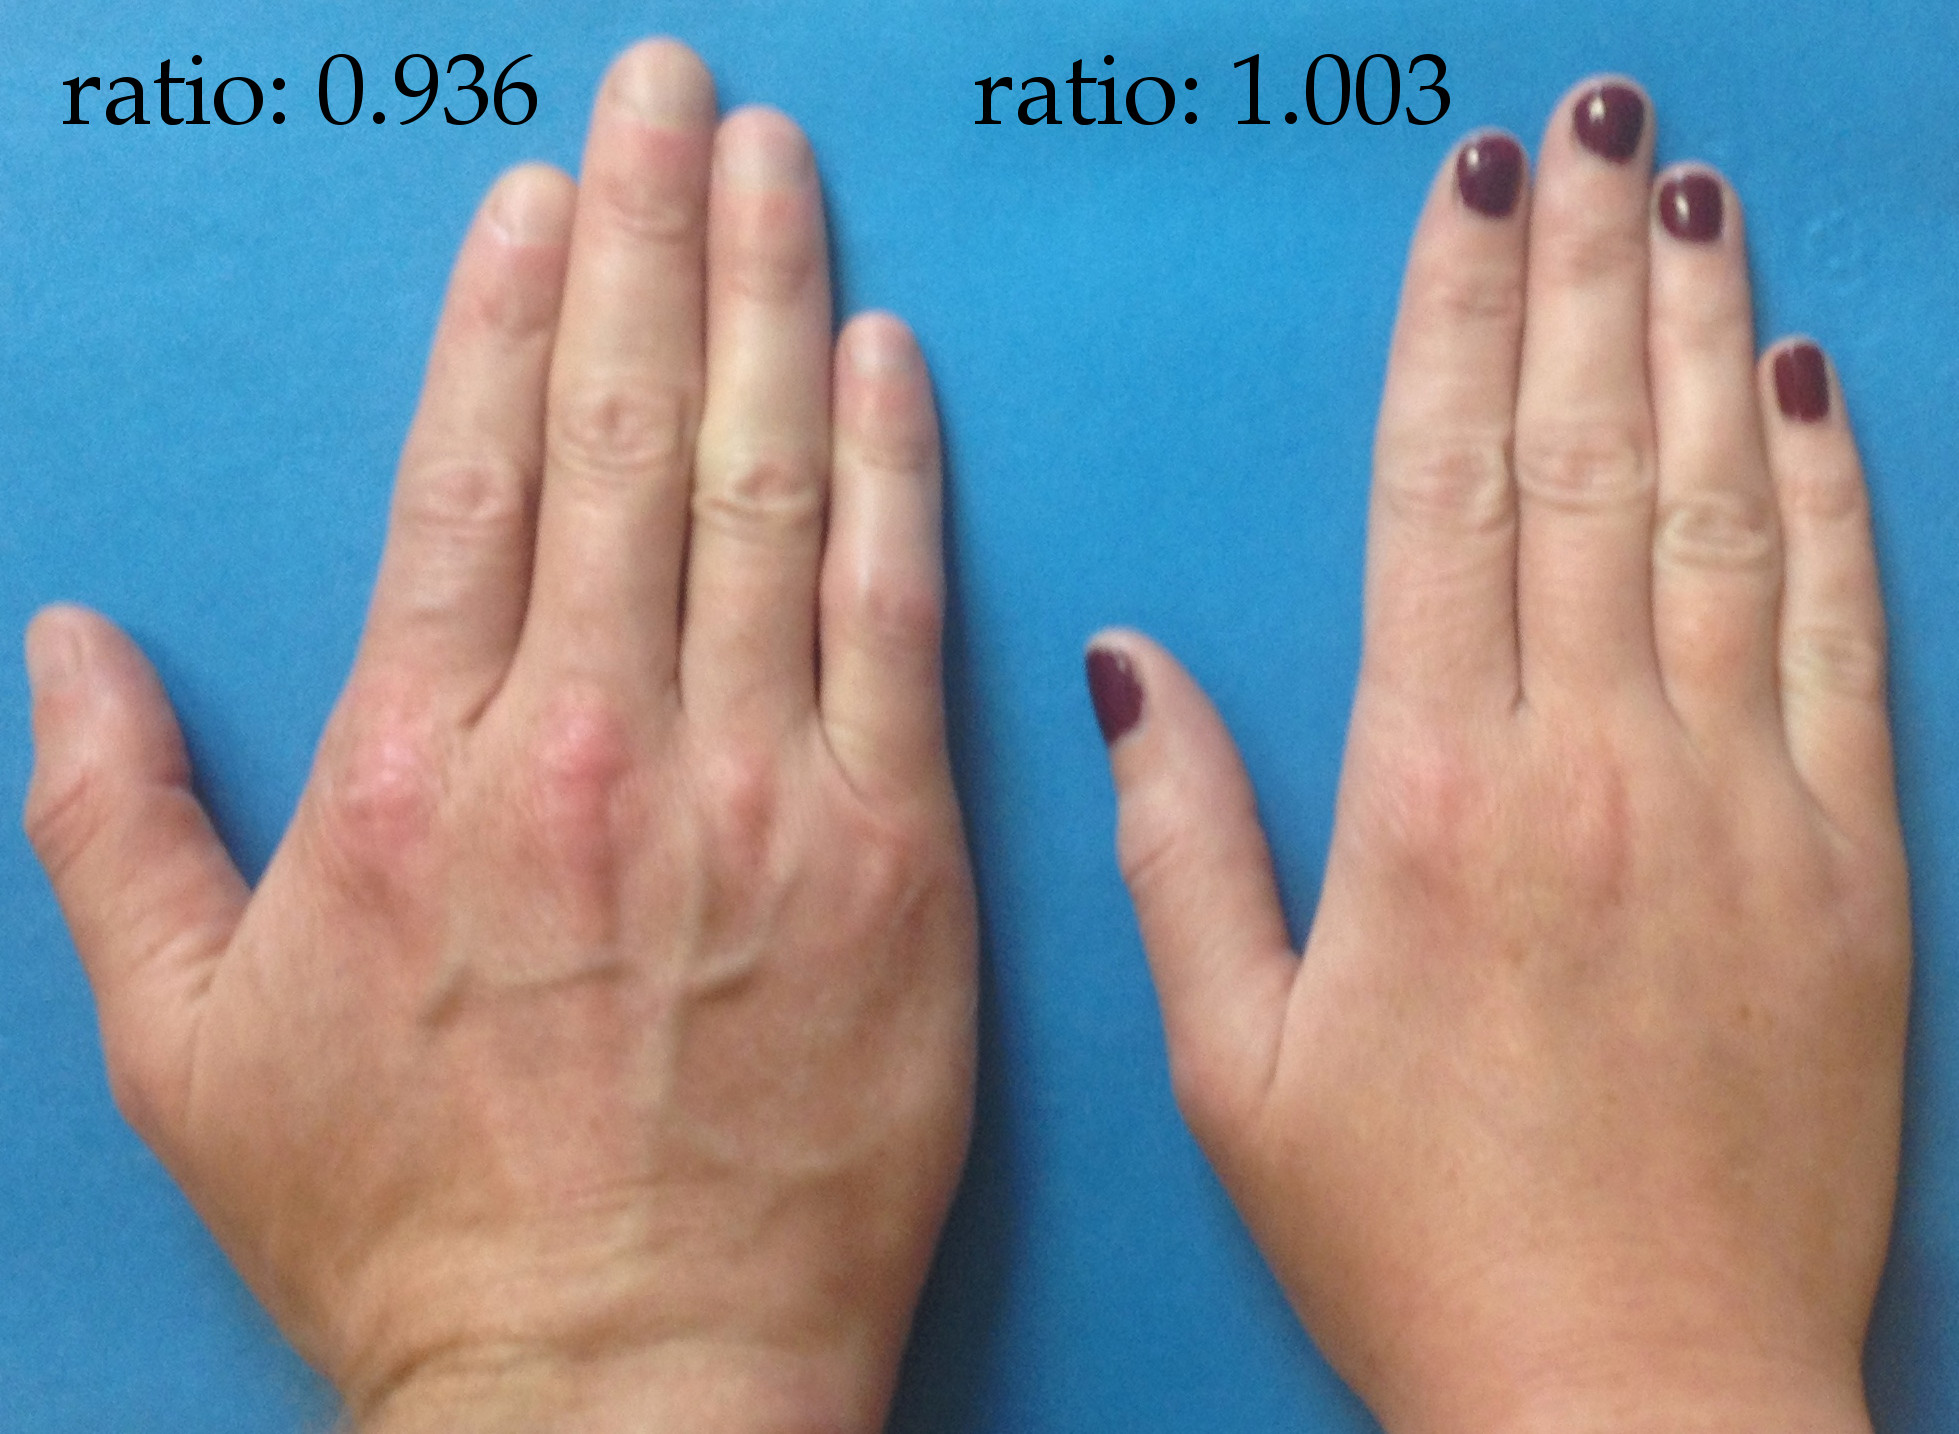
\includegraphics[width=0.6\linewidth]{realhands2.jpg}
\end{center}\vspace{1cm}


\subsection*{The Filled Pause Change in Progress}
\begin{minipage}[c]{0.70\linewidth}
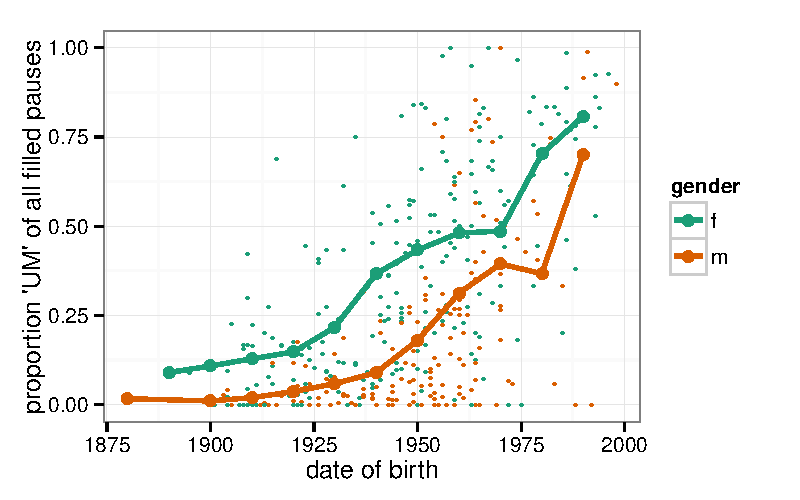
\includegraphics[width=1\linewidth]{um.pdf}
\end{minipage}
%
\begin{minipage}[c]{0.25\linewidth}
\large
When speakers use a filled pause, they are more likely to use ``um" than they used to be  (Wieling et al, \textsl{forthcoming}).
\end{minipage}




%\end{minipage}

%----------------------------------------------------------------------------------------
%	MATERIALS AND METHODS
%----------------------------------------------------------------------------------------

\section*{Results}

\begin{minipage}[c]{0.70\linewidth}
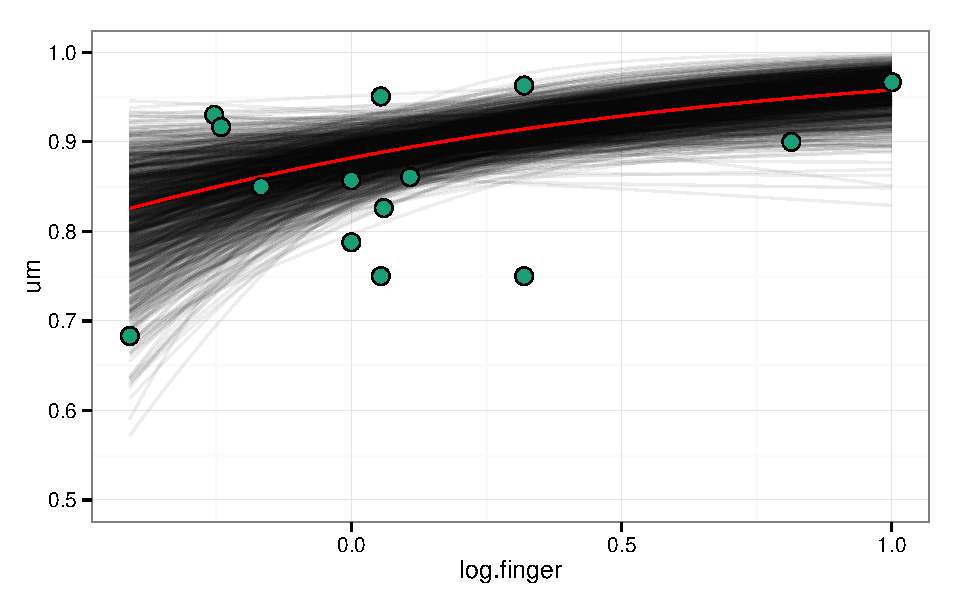
\includegraphics[width=1\linewidth]{finger_effect.pdf}
\end{minipage}
%
\begin{minipage}[c]{0.25\linewidth}
\large
Preliminary results suggest that greater 2D:4D ratio (less testosterone exposure) is correlated with more advanced UM usage.
\end{minipage}

\begin{center}
\noindent\textbf{Interpretation: less pre-natal testosterone $\rightarrow$ more \textsl{um}.}
\end{center}

\subsection*{Reliability Estimates}
1,000 bootstrap replicates produce a CI that excludes 0: (0.095,  2.567), and a permutation test (10,000 permutations) yields $p$ = 0.0563.

\begin{center}
\begin{tabular}{rrrr}
\toprule
	model & AIC & BIC & LR p-value\\
	\cmidrule{2-4}
without ratio & 813.14 & 842.64 & -- \\
with ratio &  811.36 & 845.79 & 0.052\\
\bottomrule
\end{tabular}
\end{center}

\noindent Effect size in the same order of magnitude as female effect in other spoken corpora. (Wieling et al, \textsl{forthcoming})
\begin{center}
\begin{tabular}{l r}
\toprule
\textbf{Sample} & \textbf{Effect Size}\\
\midrule
Female effect, HCRC Maptask & 2.3\\
Female effect,Fischer Corpus & 1.37\\
Female effect, PNC & 1.31\\
\textbf{Finger Ratio, our Pilot 1} & \textbf{1.12}\\
Female effect, Switchboard Corpus & 1.03\\
Female effect, British National Corpus & 0.45\\
\bottomrule
\end{tabular}
\end{center}


%\section*{Future Research}
%
%\begin{multicols}{2}
%\subsection*{Pilot Study 2}
%\begin{itemize}
%\item More Tyneside speakers.
%\item Self-report as ``tomboy''
%\item Scan 2D/4D and use digital calipers with GNU Image Modification Package \citep[][]{allawayetal2009}.
%\item A better, continuous self-report task for gender identity:
%\end{itemize}
%
%\begin{center}
%  \includegraphics[width=1\linewidth]{scale.png}
%  \end{center}
%  
%\end{multicols}
%\subsection*{Large-scale study}
%
%%ALSPAC, etc. - mostly take from Joel's York talk
%
%\begin{itemize}
%	\item As above, esp. regarding continuous gender report, but...
%	\item 200 participants from ALSPAC, with poor assays for maternal T and estradiol. 
%	\item Standard sociolinguistic interview procedures, with semi-automatic extraction of changes in progress from FAVE-aligned transcriptions:
%	\begin{itemize}
%		\item Categorical change from below: \textsl{um/uh}
%		\item Some below-consciousness phonetic and phonological variables (maybe production and perception), e.g. /uw/-fronting, pre aspiration, ...
%	\end{itemize}
%	\begin{center}
%\begin{itemize}
%\item If linguistic variables are learnt differentially depending on how masculinised brain structures have been by pre-natal androgen levels, then:
%\end{itemize}
%\end{center} 
%\begin{itemize}
%	\item Within a given sex cohort (i.e. genital-sex, or sex designated at birth), more advanced linguistic variants correspond to lower levels of pre-natal T, and perhaps other androgens (esp. women).
%	\item If the gender effect in language is purely social, then we should see no effect of hormones within each sex (only between sexes).
%\end{itemize}
%\end{itemize}
\end{multicols}
%----------------------------------------------------------------------------------------
%	CONCLUSIONS
%----------------------------------------------------------------------------------------

\color{SaddleBrown} % SaddleBrown color for the conclusions to make them stand out
\section*{Conclusions}
\begin{tabular}[b]{ll}
%\section*
%\LARGE{Conclusions}
\includegraphics[height = .17\textheight, trim={0 1cm 0 0}]{figures/possible_causes.pdf}

&
\vspace{-10cm}
%%----------------------------------------------------------------------------------------
%%	ACKNOWLEDGEMENTS
%%----------------------------------------------------------------------------------------
%
\color{DarkSlateGray}
  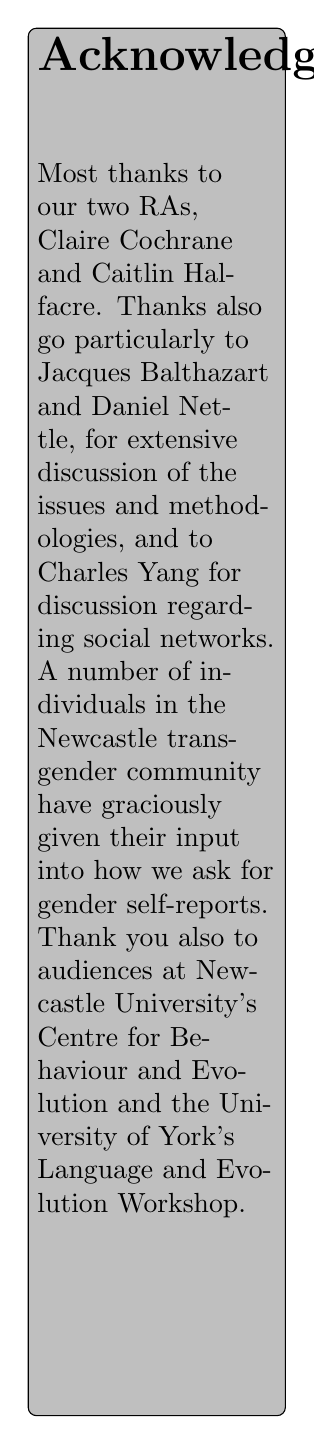
\begin{tikzpicture}
\node[draw,fill=gray!50,rectangle,text width=.25\textwidth, rounded corners=3pt] 
  {\textbf{\LARGE{Acknowledgements}}\\  \vspace{1cm} \sloppy Most thanks to our two RAs, Claire Cochrane and Caitlin Halfacre. Thanks also go particularly to Jacques Balthazart and Daniel Nettle, for extensive discussion of the issues and methodologies, and to Charles Yang for discussion regarding social networks. A number of individuals in the Newcastle transgender community have graciously given their input into how we ask for gender self-reports. Thank you also to audiences at Newcastle University's Centre for Behaviour and Evolution and the University of York's Language and Evolution Workshop. \vspace{2.4cm}
};
    \end{tikzpicture} 

\end{tabular}



 %----------------------------------------------------------------------------------------
%	REFERENCES
%----------------------------------------------------------------------------------------
\clearpage
%\nocite{*} % Print all references regardless of whether they were cited in the poster or not
\bibliographystyle{linquiry2} % Plain referencing style
\bibliography{posterrefs} % Use the example bibliography file sample.bib

%----------------------------------------------------------------------------------------


\end{document}